\documentclass[letterpaper]{article} %DO NOT CHANGE THIS

\usepackage{aaai19}    % Required
\usepackage{times}     % Required
\usepackage{helvet}    % Required
\usepackage{courier}   % Required
\usepackage{url}       % Required
\usepackage{graphicx}  % Required
\frenchspacing         % Required
\setlength{\pdfpagewidth}{8.5in}  % Required
\setlength{\pdfpageheight}{11in}  % Required

% PDF Info Is Required:
\pdfinfo{
/Title (Detecting Motifs in Knowledge Graphs using Compression)
/Author (...)}

\setcounter{secnumdepth}{0}    

\usepackage{amsmath}
\usepackage{amssymb}
\usepackage{url}
\usepackage{float}

\usepackage{easylist}
\usepackage{soul}

\newcommand{\N}{{\mathbb N}}
\newcommand{\R}{{\mathbb R}}
\newcommand{\Z}{{\mathbb Z}}

\newcommand{\X}{{\cal X}}
\newcommand{\B}{{\mathbb B}}
\newcommand{\G}{{\cal G}}
\newcommand{\cS}{{\cal S}}

\newcommand{\I}{{\cal I}}
\newcommand{\tab}{\hspace*{5mm}}
\newcommand{\from}{\leftarrow}

\floatstyle{ruled}
\newfloat{pseudo}{h}{lop}
\floatname{pseudo}{Algorithm}

\title{Detecting Motifs in Knowledge Graphs using Compression}
\author{
Author names withheld
% Peter Bloem\\
% Knowledge Representation \& Reasoning Group\\
% VU University\\
% vu@peterbloem.nl\\
}

\begin{document}

\maketitle

\begin{abstract}
\noindent We introduce a method to detect \emph{network motifs} in knowledge graphs. Network motifs are useful patterns or meaningful subunits of the graph that recur frequently. We extend the common definition of a network motif to coincide with a \emph{basic graph pattern}, commonly used in the knowledge graph literature. We introduce an approach, inspired by recent work for simple graphs, for inducing these for a given knowledge knowledge graph, and show that the motifs returned reflect the basic structure of the graph. Specifically we show that in random graphs, no motifs are found, and that when we insert a motif artificially, it can be detected, even if as few as 10 instances are inserted. Finally, we show the results of motif induction on three real-world knowledge graphs, and show that our method provides good suggestions for motifs that reflect the structure of the graph in an intuitive way.
\end{abstract}

\noindent \emph{Knowledge graphs} are an extremely versatile way of storing knowledge. They allow knowledge to be encoded without a predefined schema, they allow different amounts of data to be encoded for each known entity and they allow different modalities to be integrated seamlessly \cite{wilcke2017knowledge}. This versatility comes at a price. For a given knowledge graph, it can be difficult to see the forest for the trees: how is the graph structured at the lowest level? What kind of things can I ask of what types of entities? What are small, recurring patterns that might represent a novel insight into the data?

In the domain of unlabeled simple graphs, \emph{network motifs} \cite{milo2002network} were introduced as a tool to provide insight into local graph structure. Network motifs are small subgraphs whose frequency in the graph is unexpected with respect to a \emph{null model}. That is, for a given graph dataset $G$ and small graph $M$, we count the frequency $f(M, G)$: how often $M$ occurs in $G$ as a subgraph. We define a probability distribution over graphs $p^\text{null}(\G)$, and estimate the probability that a graph sampled from $p^\text{null}$ contains more instances of $M$ than observed in our data: $p^\text{null}(f(M, \G) \geq f(M, G))$, where $\G$ is a random variable representing a graph. If this probability is very low (commonly, below 0.05), we consider $m$ a motif. \footnotemark

\begin{figure*}[bth]
  \centering
    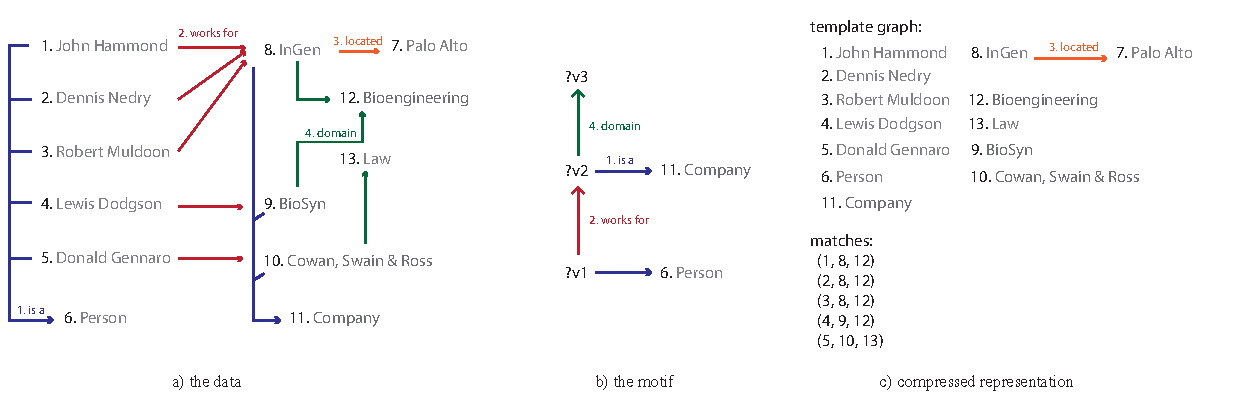
\includegraphics[width=\textwidth]{example.pdf}
    \caption{An example of the principle behind our motif code. a) A basic knowledge graph. Note that in our analysis, we consider only the indices of the nodes and relations, not their labels. b) A motif that occurs frequently. c) A compressed representation; we remove all edges that are part of an occurrence of the motif. We then store separately which nodes match the motif. The motif, together with the template graph and the matches can be used to reconstruct the graph. We take this as a heuristic: the better the motif compresses, the more characteristic it is likely to be for the graph.}
    \label{figure:example}
  \label{figure:codes}
\end{figure*}

Unfortunately, estimating this probability usually requires repeating the subgraph count on many samples from the null model. To avoid this costly operation, \cite{bloem2017large} introduces  an alternative method, using \emph{compression} as a heuristic for motif relevance: the better a motif compresses the data, the more likely it is to be meaningful. It is shown that this principle can be implemented in a similar sort of hypothesis test for a null model, allowing a comparable workflow to classical motif analysis. 

\footnotetext{This procedure has the structure of a hypothesis test, but it is important not to interpret it as \emph{statistical evidence} for the meaningfulness of the motif. The only thing it shows (in a frequentist statistical sense) is that $p^\text{null}$ is not the true source of the data. This is usually not a surprise: we are rarely able to model all aspects of a realistic data-generating process in a single distribution. The $p$-values used in motif analysis should be interpreted strictly as \emph{heuristics}. See also \cite{bloem2017large}.}

In this paper, we extend the compression-based motif analysis to knowledge graphs. For the purposes of this research we define knowledge graphs as labeled, directed multigraphs. Nodes are uniquely labeled with entity names, and links are non-uniquely labeled with relations.  We extend the definition of a motif to that of a \emph{basic graph pattern}: that is, a motif is a small graph with \emph{some} of its nodes and links labeled with entities and relations as they occur in the graph. Other nodes and links are labeled as \emph{variables}. A pattern matches at a particular location in the graph, if the variables can be replaced with values from the graph, and the motif becomes a subgraph as a result. 
The intuition behind our method is that the more compactly a pattern compresses the graph, the better the motif. Figure~\ref{figure:example} shows an illustration of the basic principle. In the preliminaries section below, we justify this intuition more formally.

We perform several experiments to show that our method returns meaningful subgraphs. First we test the intuition that a random graph shoudl contain no motifs. We also show that when we artifically insert motifs into a random graph, we can then detect these as motifs, sometimes with as few as 10 instances inserted into the graph. Finally, we show the results of motif analysis on three real-world knowledge graphs.

All code and datasets used in this paper are available, under open licenses.\footnotemark

\footnotetext{URL withheld for purposes of blind reviewing.}

\paragraph{Related Work}

Network motifs for unlabeled simple graphs were introduced in \cite{milo2002network}. A more comprehensive overview of the related literature can be found in \cite[Section~1.1]{bloem2017large}. In \cite{bloem2017large}, the principle of Minimum Description Length (MDL) was first connected to motif analysis. However, the idea had earlier been exploited for detecting meaningful subgraphs in the SUBDUE algorithm \cite{cook1994substructure}.

A few other methods have been proposed for inducing the structure of a given knowledge graph. In \cite{pham2015deriving}, the authors use the principle of characteristic sets to characterize a knowledge graph in terms of the star patterns it contains. In \cite{pham2016exploiting}, they show that the majority of the LOD cloud can be efficiently described using such principles, showing the highly tabular structure of many knowledge graphs. In \cite{volker2011statistical}, association rules mining is used to induce basic patterns in the graph. 

To the best of our knowledge, ours is the first method presented that can potentially induce any basic graph pattern.

\subsection{Preliminaries}

\paragraph{Minimum Description Length}
Our method is based on the MDL principle: that we should favour models that compress the data. We will show briefly how this intuition can be made mathematically precise. For more details, we refer the reader to \cite{grunwald2007minimum} for MDL in general, and to \cite{bloem2017large}, for a more extensive discussion these principles in the domain of graph analysis.
 
Let $\B$ be the set of all finite-length binary strings. We use $|b|$ to represent the length of $b \in \B$. Let $\log(x) = \log_2(x)$. A \emph{code} for a set of objects $\cal X$ (such as graphs) is an injective function $f: {\cal X} \to \B$, mapping objects to binary code words. All codes in this paper are \emph{prefix-free}: no code word is the prefix of another. We will denote a \emph{codelength function} with the letter $L$, ie. $L(x) = |f(x)|$. We commonly compute $L(x)$ directly, without first computing $f(x)$ and we refer to $L(x)$ as a code.

A well known result in information theory is the association between codes and probability distributions, implied by the \emph{Kraft inequality}: for each probability distribution $p$ on $\cal X$, there exists a prefix-free code $L$ such that for all $x \in \cal X$: $- \log p(x) \leq L(x) < -\log p(x) + 1$. Inversely, for every prefix-free code $L$ for $\cal X$, there exists a probability distribution $p$ such that for all $x \in \cal X$: $p(x) = 2^{-L(x)}$. For proofs, see \cite[Section~3.2.1]{grunwald2007minimum} or \cite[Theorem~5.2.1]{cover2006elements}. To explain the intuition, note that we can easily transform a code $L$ into a sampling algorithm for $p$ by feeding the decoding function random bits until it produces an output. To transform a probability distribution to a code, techniques like arithmetic coding \cite{rissanen1979arithmetic} can be used.\footnotemark 
\footnotetext{
As explained in \cite[page 96]{grunwald2007minimum}, the fact that $-\log p^*(x)$ is real-valued and $L^*(x)$ is integer-valued can be safely ignored and we may \emph{identify} codes with probability distributions, allowing codes to take non-integer values. 
}

When we need to encode a single choice from a finite set $S$ of options, we will often use the code with length $\log |S|$, corresponding to a uniform distribution on $S$. In some cases, we can allow codes with multiple codewords for a single object. If a code $L$ has multiple codewords for some object  $x$, we may indicate the choice for a particular codeword by a parameter $a$ as $L(x; a)$.

\paragraph{Relevance testing} We will use the MDL principle to perform a hypothesis test. Assume we have some data $x$ and a null hypothesis that it was sampled from distribution $p^\text{null}$. Let $L^\text{null}$ be the corresponding codelength. A simple but crucial result, known as the \emph{no-hypercompression inequality} \cite[p103]{grunwald2007minimum} tells us that the probability of sampling data $x$ from $p^\text{null}$ that can be described shorter than $L^\text{null}(x)$ by $k$ or more bits, \emph{using any code} is less than $2^{-k}$.
Thus, a standard MDL hypothesis test would consist of stating the null hypothesis in terms of a code $L^\text{null}$, designing a code (before seeing the data) which compresses the data better than $L^\text{null}$ by, say, 10 bits and rejecting the null hypothesis with confidence $2^{-10}$. For a longer, more intuitive explanation of this principle in pattern induction, we refer the reader to \cite[Section~2]{bloem2017large}.

We must note again, that when we use this procedure to find motifs, we are not providing evidence for the hypothesis that the motif is ``correct.'' The only thing we are statistically proving is that the null-model is incorrect. Nevertheless, hypothesis testing has shown to be a valuable heuristic in motif analysis.

\paragraph{Common codes}
In the construction of our codes for graphs, we require some simpler codes as building blocks. First, when we store any positive integer $n$, we do so with the code corresponding to the distribution $p^\N(n) = 1/(n(n+1))$, and denote it $L^\N(n)$. For nonnegative numbers we add 1 to the argument. for the full range of integers, we add an extra bit for the sign, and then use the first code for negative integers and the second for positive ones.

We will often need to encode sequences of integers. These will be highly skewed, with only a subset of integers occurring frequently, and others occurring infrequently or not at all. As noted in \cite{de2016names} a code based on the Pitman-Yor model \cite{pitman1997two} is very effective in such situations. Let $S = \langle S_1, ..., S_n\rangle$ be a sequence of integers of length $n$. We first store its members $m(s)$ in the order in which they first occur: we first store $n$ and the first member using the codes described above. The rest of the members are stored sequentially using the distance from the current to the next member.

Let $f(A, B)$ be the frequency of symbol $A$ in sequence $B$.We then store the complete sequence using the code corresponding to the following distribution:
\begin{align*}
&p^\text{PY}_{\alpha,d}(S) = \prod_{i \in [1,k]} \text{PY}_{\alpha,d}(S_i\mid S_{1:i-1}) \\
&\text{PY}_{\alpha,d}(S_i \mid S') = 
\begin{cases}
\frac{\alpha - d |m(S)|}{|m(S)| + \alpha} & \text{if} f(S_i, S') = 0 \\ 
\frac{f(S_i, S') - d}{|m(S)| + \alpha} & \text{otherwise}
\end{cases}
\end{align*}
See \cite{de2016names} for a more intuitive explanation. In all experiments we use $\alpha = 0.5$, $d=0.1$. We will refer to the total for a sequence  codelength under this procedure as $L^PY(S)$

\section{Method}

We will start with some formal definitions of our basic ingredients. To comfortably define probabilities and codes on graphs, we will slightly deviate from conventional definitions. Specifically, we will analyse the \emph{structure} of knowledge graphs only, ignoring any meaning they have outside the graph. For instance, we will distinguish between links with different labels, but we will ignore any internal structure of the label itself (such as shared IRI prefixes). Under this assumption we can assume that the node and link labels of our knowledge graphs are simply natural numbers.\footnotemark This leads to the following definition.

\footnotetext{For practitioners this restriction is not noticeable, as the indices can simply be mapped back to the original strings when the found motifs are presented.}

A \emph{knowledge graph} $G$, hereafter simply a \emph{graph}, is a tuple $G = (v_G, r_G, E_G)$. $v_G \in \N$ is the number of nodes in the graph, and $r_G \in \N$ is the number of relations. We define the nodeset as $V_G = \{0, \ldots, v_G-1\}$ and the relation-set as $R_G = \{0, \ldots, r_G\}$. The \emph{tripleset} $E_G \subset V_G \times R \times V_G$ determines the edges of the graph and their labels. 

As shown in Figure~\ref{figure:example}, the patterns that we aim to find are partially labeled: some nodes and edges are labeled with as variables. We will represent these with negative integers. A pattern $M$ for graph $G$ is a tuple $(V_M, R_M, G, E_M)$. Let $v_M$ and $r_M$ indicate the number of variable nodes and variable links in $M$ respectively, then $V_M \subseteq \{-v'_M, \ldots, v_G-1\}$ and $R_M \subseteq \{-(r'_M+v'M), \ldots,-v'M, 0,\ldots, r_G-1\}$, with $E_M \subset V_M \times R_M \times V_M$, as for regular graphs. That is; nodes can be labeled either with nonnegative integers referring to $G$'s nodes or with negative integers representing a variable node, and similar for relations. The negative integers are always contiguous within a single graph, with the highest representing the node labels and the lowest representing the edge labels.

An \emph{instance} for $M$ in $G$ is a pair of sequences of integers: $I = (I^n, I^r)$. $I^n$ is a sequence of distinct integers of length $v'_M$. $I^r$ is a sequence of non-distinct integers of length $r'_M$. For each edge $(s, p, o) \in E_M$ containing a negative $s$, $p$ or $o$, there is a corresponding link in $E_G$ with a negative $s$ replaced by $I^n_{-s}$, a negative $o$ replaced by $I^n_{-o}$, and a negative $p$ replaced by $I^r_{-p - v'_M}$. Put simply: for a pattern to match, variable edges marked with the same negative integer, must map to the same relation in order for the pattern to match, but variable links labeled with different negative integers \emph{may} map to the same relation. Variable nodes are always labeled distinctly and may never map to the same node in $G$. An instance describes a subgraph of $G$ that \emph{matches} the pattern $M$. Each edge in the motif may only match one edge in the graph. In other words, the occurrence of the motif in the graph must have as many edges as the motif itself.

We will first assume that a target pattern $M$ is given for the data $G$ and that we have a set of instances $\I$. Moreover, we require that all instances in $\I$ are mutually disjoint: no two subgraphs defined by member of $\I$ may share an edge, but nodes may be shared. In most settings we do not actually have a given $M$ and $\I$ and we will need to search for them. We describe a simple and search algorithm in Section~\ref{section:search}.

\label{section:relevance-test}

\section{Null model}

\label{section:null-model}

The most common null model for classical motif analysis is the degree-sequence model (also known a the configuration model \cite{newman2010networks}): a uniform distribution over all graphs with a particular degree sequence. We extend this to knowledge graphs by also including the degree of each relation: that is, the frequency with which it occurs in the tripleset. Let a \emph{degree sequence} $D$ of length $n$ be a triple of three integer sequences: $(D^\text{in}, D^\text{rel}, D^\text{out})$. If $D$ is the degree sequence of a graph, then node $i$ has $D^\text{in}_i$ incoming links,  $D^\text{out}_i$ outgoing links and for each relation $r$, there are $D^\text{rel}_r$ triples.

Let $\G_D$ be the set of all graphs with degree sequence $D$. Then the configuration model can be expressed simply as
\[
p^C(G) = \frac{1}{|\G_D|}
\]
for any $G$ that satisfies $D$ and $p(G) = 0$ otherwise. Unfortunately, there is no efficient way to compute $|\G_D|$ and even approximations tend to be costly for large graphs. Following the approach in \cite{bloem2017large}, we define a fast approximation to the configuration model, which works well in practice for motif detection. 

We can describe a knowledge graph by three length-$m$ integer sequences: $S$, $P$, $O$, such that $\{(S_j, P_j, O_j)\}_j$ is the graph's tripleset. If the graph satisfies degree sequence $D$, then we know that $S$ should contain node $j$ $D^\text{out}_j$ times, $P$ should contain relation $r$ $D^\text{rel}_r$ times and $O$ should contain node $j$ $D^\text{in}_j$ times.  Let ${\cal S}_D$ be the set of all such triples of integer sequences satisfying $D$. We have 
\[
|{\cal S}_D| =
 {m \choose {D_1^\text{out}, \ldots, D_n^\text{out}} }
 {m \choose {D_1^\text{rel}, \ldots, D_{|R_G|}^\text{rel}} }
 {m \choose {D_1^\text{in}, \ldots, D_n^\text{in}} } \text{.}
\]

While every member of ${\cal S}_D$ represents a valid graph satisfying $D$, many graphs are represented multiple times. Firstly, many elements of ${S}_D$ contain the same link multiple times. We call the set without these elements ${\cal S'}_D \subset {\cal S}_D$. Secondly the links of the graph are listed in arbitrary order; if we apply the same permutation to all three lists $S$, $P$ and $O$, we get a new representation of the same graph. Since we know that any element in ${\cal S}'_D$ contains only unique triples, we know that each graph is present exactly $m!$ times. This gives us
\[
|\G_D| = |{\cal S}'_D| \frac{1}{m!} \leq  |{\cal S}_D| \frac{1}{m!} \text{.}
\]

We can thus use 
\[
p^\text{EL}_D(G) =  \frac{m!}{{m \choose {D_1^\text{out}, \ldots, D_n^\text{out}} }
 {m \choose {D_1^\text{rel}, \ldots, D_{|R_G|}^\text{rel}} }
 {m \choose {D_1^\text{in}, \ldots, D_n^\text{in}} }} \leq p^C(G) \text{.}
\]

Filling in the definition of the multinomial coefficient, and rewriting, we get a codelength of:
\begin{align*}
- &\log p^\text{EL}_D(G) = 2 \log(m!) \\
&- \sum_i \log(D_i^\text{in}!)- \sum_i \log(D_i^\text{rel}!)- \sum_i \log(D_i^\text{out}!)
\end{align*}

as an approximation for the DS model. We call this the edgelist (EL) model. It gives a probability that always lower-bounds the configuration model, since it affords some probability mass to graphs that cannot exist.\footnotemark ~Experiments in the classical motif setting have shown that the EL model is an acceptable proxy for the DS model \cite{bloem2017large}, especially considering the extra scalability it affords.

\footnotetext{Note that we cannot simply think of $p^\text{EL}$ as a uniform model for graphs containing multiple links, since we can only divide by $m!$ if we know that all triples are unique.}
 
 \paragraph{Encoding D} In order to encode a graph with $L^\text{EL}_D$, we must first encode $D$. \footnote{Or, equivalently, to make $p^\text{EL}$ a complete distribution on all graphs, we must provide it with a prior on $D$.} For each of the three sequences in $D$ we use the following model:
\begin{align*}
 p(D) &= \prod_i q^{\N}(D_i) \\
 L(D) &= - \sum_i \log q^{\N}(D_i)
\end{align*}

where $1^{\N}$ is any distribution on the natural numbers. This is an optimal encoding for $D$ assuming that its members are independently drawn from $q^{\N}$. When we use $p^\text{EL}$ as the null model, we use the data distribution for $q^{\N}$ to ensure that we have a lower bound to the optimal code-lengthn (in essence, we cheat, giving the null model a slightly lower than optimal codelength). When we use $p^\text{EL}$ as part of the motif code, we must use a fair encoding, so we use the Pitman-Yor code to store each sequence in $D$.

In the design of our method, we will constantly aim to find a trade-off between completeness and efficiency that allows the method to scale to very large graphs. Specifically, when we economize, we will only do so in a way that makes the hypothesis test \emph{more conservative}.

\subsection{Motif code}

As described above, we can perform our relevance test with any compression method which exploits the pattern $M$, and its instances $\I$ to store the graph efficiently. The better our method, the more motifs we will find. Note that there is no need for our code to be optimal in any sense. So long as we accept that we won't find all motifs that exist, we are free to trade off compression performance against efficiency of computation.

We store the graph by encoding various aspects, one after the other. The information in all of these together is sufficient to reconstruct the graph. Note that everything is stored using prefix-free codes, so that we can simply concatenate the codewords (or rather, sum the codelengths we get for each aspect).

We also assume that we are given a code $L^\text{base}$ for generic knowledge graphs (in practice, this will be the null model, although the motif code is valid for any base code).

We store, in order:

\begin{description}
 \item[the graph dimensions] We first store $|V_G|$, $|E_G|$ and $|R_G|$ using the generic code $L^{\N}(\cdot)$. 
 \item[the pattern] We store the structure of the pattern using the base code, and its labels as a sequence using the Pitman-Yor code.
 \item[the template] This is the graph, minus all links occurring in instances of $M$. Let $E_G'$ be $E_G$ minus any link occurring in any member of $\cal I$. We then store $(V_G, E_G')$ using $L^\text{base}(\cdot)$.
 \item[the instances] To store the instances, we view the connections between the nodes made by motifs as a hypergraph, and we extend the EL code to store it. The details are given below.
\end{description}

The precise computation of the codelength is given in Algorithm~\ref{algorithm:motif-code}. 

We note a few aspects of this code. Firstly, it achieves its compression by reducing the number of links it has to store. For each additional instance, it pays the cost of storing the instance, and any variable nodes and links, but it saves $|E_M|$ links in storing the template. The precise trade-off depends on the choice of base code, and on the structure of the rest of the graph (some edges are cheaper to store than others, for some codes).

Nevertheless, we can make a few broad observations: patterns with many variable nodes and links are more costly to store than fully labeled patterns. On the other hand, a pattern with many variable nodes and links is more likely to have many instances, so that \emph{if} it results in a small amount of compression per instance, the large number of instances may cause it to compress a lot. For the variable nodes and links, we use a DM model for each specific node and link. This means that the more structure there is to the label given to a particular part of the pattern, the better we compress. For instance, suppose a particular node of the pattern is always labeled with either a node corresponding to YES or NO, in equal proportion, we will require only a bit per instance to record those labels. If, however, all nodes in the graph are equally likely to appear in the position of the variable, we will pay approximately $\log |V_G|$ bits per instance. If only a single node appears in the position, we pay only a a constant number of bits to record the entire sequence of instances. Thus, to our code, non-variable nodes are just a highly regular type of variable node. The distinction is only meaningful in the search algorithm.

\begin{pseudo}[tb]
\caption{The motif code $L^\text{motif}(G ; M, {\cal I}, L^\text{base})$. Note that the nodes and relations of the graph are integers.}
\label{algorithm:motif-code}
{ 
\textbf{function} $\text{codelength}(G; M, {\cal I}, L^\text{base})$:\\
\tab\tab a graph $G$, a pattern $M$\\ 
\tab\tab instances $\cal I$ of $M$ in $G$, a code $L^\text{base}$.\\
\\
$b_\text{dim} \leftarrow L^\N(|V_G|) + L^\N(|R_G|) + L^\N(|E_G|)$ \\

\emph{\# Turn the pattern into a normal knowledge graph}\\
$E_{M'} \leftarrow$ the edges of $M$ with contiguous integer labels \\
$M' \leftarrow (|V_M|, |R_M|, E_{M'})$ \\
$S_M \leftarrow$ the labels of M in canonical order \\
$b_\text{pattern} \leftarrow L^\text{base}(M') + L^{PY}(S_M) $\\

\emph{\# Store the template graph}\\
$E'_G \leftarrow E_G - \cup_{\I \in {\cal I}} \text{triples}(I)$ \\
$b_\text{template} \leftarrow L_\text{base}((V_G, R_G, E'_G))$\\

$b_\text{instances} \leftarrow -\log p_M(\I) + \sum_{D \in D^{\I}} L^{PY}(D)$\\

\textbf{return} $b_\text{dim} + b_\text{pattern} + b_\text{template} + b_\text{instances}$\\
}
\end{pseudo} 

\subsection{Encoding motif instances}

To encode a list of instances $\I$ of a given pattern $M$, we generalize  the idea of the edgelist model described above. To understand the following ,it may be instructive to think of a single triple as an instance for the pattern
\[
\texttt{?n1 ?rel ?n2}.
\]
 We can now think of the edgelist model as storing a sequence of instances for this pattern, which together make up the entire knowledge graph.
 
 To generalize this notion to arbitrary patterns, to be defined for a given template graph, we define the \emph{degree constraint} $D^\I$ of a list of instamces for a given pattern as follows: for each variable node $i$ in the pattern, the degree sequence provides an integer sequence $D^i$ of length $v_G$, indicating how often each node in the completed knowledge graph takes that position in the pattern. Similarly, for each variable link $j$ in the pattern, the degree sequence provides an integer sequence $C^j$ of length $r_G$ indicating for each relation how often it takes that position in the pattern.
 
 We store these sequences in the same manner as the degree sequence of the template graph, using the Pitman-Yor code for each.
 
Given this information, all we need to do is describe which of the possible sequences of matches for this pattern satisfying the given degree sequence we are encoding. As with the configuration model, the ideal is a uniform code over all possible configurations, for which we will define an approximation. Given $w$ variable nodes in a pattern, and $l$ variable links, we can define such a collection of instances using $w+l$ integer sequences: $N^1, \ldots, N^n, L^1, \ldots, L^l$, with the $t$-th instance defined by the integer tuple $(N^1_t, \ldots, N^n_t, L^1_t, \ldots, L^l_t)$. If this set of sequences satisfies the degree constraint, we know that node $q$ must occur $D^i_q$ times in sequence $N^i$, and similarly for the variable links. Let $\cS_\I$ be the set of all such integer sequences satisfying the degree constraint. We will follow the same logic as for the EdgeList model. Let $k$ be the number of matches of the pattern. We have:
\begin{align*}
|\cS| = &{k \choose D^1_1, \ldots, D^1_v}\times \ldots \times{k \choose D^w_1, \ldots, D^w_v}\times \\
&{k \choose C^1_1, \ldots, C^1_r}\times \ldots \times{k \choose C^l_1, \ldots, C^l_r}
\end{align*}

As before, this set is larger than the set we are interested in. First, each set of pattern matches is contained multiple times (once for each permutation) and second, not all elements are valid pattern matches (in some, a single triple may be represented by multiple instances). Let $\cS_\I'$ be the subset representing only valid matches, and let $\G_\I$ be the set of valid instances with permutations removed. As before, we have
\[
|\G_\I| = |\cS'_\I| \frac{1}{k!} \leq  |\cS_\I| \frac{1}{k!} \text{.}
\]
Which gives us the following distribution
\[
p_M(G) =  \frac{k!}{|\cS_D|} < \frac{1}{\G_D} \text{,}
\]
 with $-\log p_M(\I)$ as a code to store the instances. Rewriting as before, gives us a codelength of 
 \begin{align*}
 - \log p_M(G) &= (w+l-1)\log(k!) \\
  -&\sum_{j\in [1,w], i} \log(D^j_i!) -\sum_{j\in [1,l], i} \log(C^j_i!)
 \end{align*}
 
Note that if we store a graph with the pattern $\texttt{?n1 ?rel ?n2.}$, we obtain an empty template graph, and the motif code achieves the same codelength as the edgelist model, up to a small constant amount for storing the pattern.
 

For a given graph and pattern, we can simply find the complete list of instances using a graph patter search. Since we require a slightly different semantics than standard graph pattern matchers, we adapt the DualIso algorithm \cite{saltz2014dualiso} for knowledge graph matching. Before computing the motif code, we prune the list of instances provided by this search iterating over the instances and removing and instance that produces a triple also produced by an earlier instance.

Since graph matching encompasses subgraph isomorphism, it is known to be NP-Complete. To guard against rare patterns that produce long-running searches we terminate all searches after 5 seconds, returning  only those matches that were found within the time limit.

We express the strength of a motif by its log-factor: $-\log p^\text{null}(G) + \log p^\text{motif}(G; M, \I, L^\text{base})$. If this value is positive, the motif code compresses the graph better than the null model. If the log-factor is greater than 10 bits, it corresponds to a rejection of the null model at $p < 0.001$.

\subsection{Motif search}

\label{section:search}

Ultimately, we want to find any motifs that have a high log-factor for a given graph $G$. Since we can readily compute the log-factor, any black-box optimization algorithm can be used to search the space of all possible motifs. For the sake of simplicity, we will use basic simulated annealing here. The starting pattern is always a single random triple from the graph, with its relation made a variable. We define seven possible transition from one pattern to another:
\begin{description}
	\item[Extend (0.1)] Choose an instance of the pattern and an adjacent triple not part of the instance. Add the triple to the pattern.
	\item[Make a node a variable (3)] Choose a random constant node, and turn it in to a variable node.
	\item[Make an edge a variable (3)] Choose a random constant edge label, and turn it in to a variable (always introducing a new variable).
	\item[Make a variable node constant (2)] Choose a random variable node and turn it into a constant. Take the value from a random instance.
	\item[Make a variable edge constant (2)] Choose a random variable edge and turn it into a constant. Take the value from a random instance.
	\item[Remove edge (3)] Remove a random edge from the pattern, ensuring that it stays connected.
	\item[Couple (1)] Take two distinct edge variables, which for at least one instance hold the same value and turn them into a single variable.
\end{description}

The values in brackets are the relative weights of each transition type (chosen by trial and error to keep the algorithm stable). We choose a transition at random and compute a new pattern. If the transition cannot be made (for instance, there are no constant node to make variable) or if the resultant pattern is in some way invalid, we sample a new transition.

Once a new pattern has been sampled, we compare its codelength under the motif model to that of the previous sample. If the codelength is lower, we continue with the new pattern. If the codelentgh is longer, we continue with the new sample with probability $\alpha$ or return to the previous pattern otherwise. We use $\alpha = 0.5$ in all experiments.

We store all patterns seen and their scores. In order to exploit all available processor cores, we run several searches in parallel. After each the searches are finished, we tajke the top 1000 patterns from each and sort them by motif codelength. If two searches return different codelengths\footnotemark for a motif we take the lowest value.
 
\footnotemark{This is possible if the pattern search is cut off due to the 5 second time limit.}
 
\section{Experiments}

To validate the method, we first test it on random graphs. We sample a directed graph with a given number of nodes $n$ and edges $m$, with no self-connections and multiple edges (that is, we sample from from the $G(n, m)$ Erd\H{o}s-Renyi model). We then label the nodes uniformly at random with one of the relations in $0, \ldots, r$. To make the dimensions realistic we base them on thos of the Mutag dataset used later: $n=23644$, $m74567$, $r=24$.

We then take one randomly chosen pattern, and insert $k$ instances of the pattern into the graph. We run the experiment for $k=0$, $k=10$ and $k=100$.

\section{Acknowledgments}

Withheld for purposes of blind reviewing.
% This publication was supported by the Amsterdam Academic Alliance Data Science (AAA-DS) Program Award to the UvA and VU Universities. 

% References and End of Paper
\bibliography{kgmotifs}
\bibliographystyle{aaai}


\end{document}
